\documentclass{article}
\usepackage[final]{neurips_2026}
\usepackage[utf8]{inputenc}
\usepackage[T1]{fontenc}
\usepackage{hyperref}
\usepackage{url}
\usepackage{booktabs}
\usepackage{amsfonts,amsmath}
\usepackage{nicefrac}
\usepackage{microtype}
\usepackage{graphicx}

\title{Shared-Label Item Response Models with a Learned Second Stage for the Predictive AI Evaluation Competition}

\author{%
  Komi Denis Atoukouvi \\
  ENSEA, Abidjan, C\^ote d'Ivoire \\
}

\emergencystretch=3em
\begin{document}
\maketitle

\begin{abstract}
We describe our entry to the NeurIPS 2026 Predictive AI Evaluation Competition (PAIEC), where a predictor must output the probability that an AI system answers a benchmark item correctly, given a small and growing budget of labels revealed at test time (0, 1, 3, 7, 15 and 31 labels per subject--benchmark pair). The score is the Brier area under the label curve (Brier ALC). Our final submission is a small, dependency-free Python model. For each benchmark it fits a regularised logistic item response model, $\mathrm{logit}\,p = c + a_{s} + d_{j}$, on every label that the evaluator reveals for that benchmark, including labels of \emph{other} subjects, and it estimates the strength of its two prior scales from the data (empirical Bayes). A small tree ensemble, trained offline on simulated episodes built from the public data and validated by holding out whole benchmarks, then corrects the item response probabilities using their uncertainty, the coverage of the item and the number of labels. In our offline simulation of the evaluator shared labels improve the Brier ALC by 0.011 to 0.030 over a per-pair shrinkage baseline, and the second stage adds a further 0.0004 to 0.0026 that only uses the target subject's own labels. The Codabench feedback phase is too noisy to confirm such differences: resubmitting the identical file gave scores from 0.153 to 0.195 (v3) and from 0.175 to 0.200 (v4), so we selected the model on the simulation, not on the leaderboard. We also report the ideas that did \emph{not} help in our simulations: text embeddings of items, priors based on model names, low-rank latent factors, label acquisition policies and a tuned constant for the zero-label case.
\end{abstract}

\section{Task and scoring}
\label{sec:task}
A predictor implements \texttt{predict(input, labeled)} and receives a subject (an AI system with metadata), an item (with text and a benchmark identifier) and the list \texttt{labeled} of revealed labels. For each subject--benchmark pair the evaluator reveals up to 31 labels, in nested sets of size $b\in\{0,1,3,7,15,31\}$, and scores the prediction on held-out items of that pair with the Brier score \citep{brier1950}. The final metric is
\[
\text{Brier ALC} = 0.1\,B_0 + 0.2\,B_1 + 0.2\,B_3 + 0.2\,B_7 + 0.2\,B_{15} + 0.1\,B_{31},
\]
averaged over pairs, lower being better. Predicting $0.5$ always gives $0.25$. The competition rules state that \texttt{labeled} contains \texttt{[[subject, item], label]} entries gathered across the sampled subject--benchmark pairs, that is, labels of other subjects and benchmarks are visible to the predictor. This observation drives our whole approach: the labels of other subjects on the same benchmark are informative about item difficulty, which a predictor that sees only its own pair cannot learn.

\section{Data and validation protocol}
\label{sec:data}
\paragraph{Training data.} We use only the public \texttt{measurement-db} collection (Hugging Face dataset \texttt{aims-foundations/\allowbreak measurement-db}). We kept every benchmark whose responses are all in $\{0,1\}$ (170 benchmarks, 69.2 million response rows) and discarded non-binary ones. No other training data was used, and the submitted model does not call any external model or service.

\paragraph{Offline simulation of the evaluator.} The hidden test is not available, and the Codabench leaderboard is not visible, so we built a simulator of the protocol. For every (subject, benchmark) pair with at least 80 distinct items, items are split at random into an acquisition pool and an evaluation pool (50/50, independently per pair). The first $b$ items of the acquisition pool, in a fixed random order, play the role of the revealed labels. The prediction is scored on up to 200 evaluation items of the pair against the item's mean response over trials, using the Brier score. After the eligibility filters (at least 31 acquisition labels and 10 evaluation items) the simulation uses 13,238 pairs from 154 benchmarks. The simulation includes a knob $S$, the number of subject--benchmark pairs of the same benchmark whose labels are visible to the predictor (10, 30, 100, or all pairs of the benchmark), because the real number is unknown to us. Benchmarks with at most $S$ eligible pairs are skipped for that $S$, so the benchmark set changes with $S$ and the columns of Table~\ref{tab:sim} are not strictly comparable with each other.

\section{Methods}
\label{sec:methods}
We built four successive versions. All are pure Python without third-party packages and predict $0.5$ when no label of the benchmark is available.

\paragraph{v1: per-pair shrinkage.} With $k$ successes among the $n$ revealed labels of the target subject on the target benchmark, $\hat p=(k+1)/(n+2)$. Two refinements (a prior from the subject's name, and tuning of the strength per budget by leave-benchmark-out cross-validation) did not improve on this and were disabled in the submitted parameters.

\paragraph{v2: shared-label item response model.} Following the Rasch model \citep{rasch1960}, for the benchmark of the query, we collect every revealed label of that benchmark, whatever the subject, and fit
\[
\mathrm{logit}\,P(y_{sj}=1) = c + a_s + d_j,\qquad a_s\sim\mathcal N(0,\tau_a^2),\; d_j\sim\mathcal N(0,\tau_d^2),\; c\sim\mathcal N(0,1.5^2),
\]
where $s$ indexes subjects and $j$ items. The posterior mode is computed by cyclic Newton updates of $c$, of all $a_s$ and of all $d_j$ (20 sweeps, diagonal Hessians), which is fast enough in pure Python (about 2 seconds for 60{,}000 labels). Subjects and items are identified by their serialised metadata, so an item seen only in another subject's labels still receives a difficulty. For an item without revealed label the difficulty is $0$. Predictions are clipped to $[0.02,0.98]$ and fits are cached per (benchmark, number of labels). The prior scales were $\tau_a=1.0$ and $\tau_d=1.5$. Without labels of other subjects the model reduces to a smoothed success rate of the target pair.

\paragraph{v3: empirical Bayes prior scales.} The best fixed scales depend on how many subjects are visible (Table~\ref{tab:sim}), which we do not know for the hidden test. Version 3 therefore re-estimates $\tau_a$ and $\tau_d$ from the fit itself. Starting from $(1.25, 2.0)$, after a burn-in of four sweeps and then every second sweep, we set
\[
\tau_a \leftarrow \operatorname{clip}\Big(\sqrt{\tfrac1{n_S}\textstyle\sum_s (a_s^2 + h_{a,s}^{-1})},\,0.6,\,3\Big),
\]
and similarly for $\tau_d$, where $h$ is the diagonal posterior precision (24 sweeps in total). This is the usual EM update for a normal prior scale (see \citealp{efron1973stein}). On the simulation the estimated scales were about $0.7$--$0.9$ for subjects and $1.0$--$1.3$ for items.

\paragraph{v4: learned second stage.} The item response model is parametric and can be systematically miscalibrated: it ignores the discrimination of items, it treats the difficulty of an unlabelled item as exactly zero, and it does not know how reliable a fit is. We therefore train a second stage that maps the stage-one output and a few diagnostics to a corrected probability, in the spirit of the combined estimators of \citet{polo2024tiny}. For each query it uses 20 features computed from the fit: the logit $\eta$ and its two parts $c+a_s$ and $d_j$; whether the item has a revealed label (from any subject) and how many; the posterior variances of $a_s$ and $d_j$ (the prior variance $\tau_d^2$ for an unlabelled item); the number of labels of the target subject and its smoothed success rate; the number of visible subjects and the mean number of labels per subject; the base rate of the benchmark; the two estimated prior scales; the shrunk empirical success rate of the item; and five first-order two-parameter-logistic signals, namely one Newton step for an item slope and for a subject slope, their products with $a_s$ and $d_j$, and the mean residual of the item (Appendix~\ref{app:impl}). The learner is a gradient-boosted regression-tree ensemble with squared-error loss, hence directly the Brier score (120 trees, depth 4, at least 200 rows per leaf, $\ell_2$ penalty 1; no tuning). It is trained on 3.36 million rows from the simulator of Section~\ref{sec:data} (every benchmark, $S\in\{10,30,100,\text{all}\}$, budgets 1 to 31, 40 evaluation items per pair) and exported as a 170~kB JSON file that the pure-Python \texttt{model.py} evaluates. The prediction at budget 0, or for a subject without any label on the benchmark, is the stage-one probability.

\paragraph{Label acquisition.} We submit no \texttt{labeling.py}, so the evaluator's default random policy is used (Section~\ref{sec:negative}).

\section{Results}
\label{sec:results}
\paragraph{Codabench feedback phase.} Table~\ref{tab:real} gives the scores returned by Codabench. The feedback score is computed on a newly sampled subset of the hidden data, and it is very noisy: the same v3 file, submitted three times within a few minutes, scored 0.170854, 0.153215 and 0.194889, and the final v4 file, submitted five times, scored 0.175236, 0.195902, 0.200398, 0.189295 and 0.186199 (mean 0.1894, standard deviation 0.0102). These spreads (0.04 for v3 and 0.025 for v4) are larger than the differences between our versions, and the five v4 scores average higher than the three v3 scores (0.1730), a difference of 0.016 that is well inside this noise (about 1.3 standard errors). The feedback scores therefore cannot rank our versions, in either direction. We therefore chose the final model with the simulation of Section~\ref{sec:data}, where all methods are evaluated on the same 13{,}238 pairs, and we report the Codabench numbers only for transparency.

\begin{table}[h]
\centering
\caption{Codabench feedback scores (Brier ALC, lower is better). Each row is one submission; the three v3 rows are the same file, and so are the five v4 rows.}
\label{tab:real}
\begin{tabular}{llr}
\toprule
Version & Method & Score \\
\midrule
v1 & per-pair shrinkage, $(k+1)/(n+2)$ & 0.195943 \\
v2 & shared-label IRT, fixed scales (1.0, 1.5) & 0.171685 \\
v3 & shared-label IRT, empirical Bayes scales & 0.170854 \\
v3 (same file) & resubmission 1 & 0.153215 \\
v3 (same file) & resubmission 2 & 0.194889 \\
v4 & shared-label IRT with second stage & 0.175236 \\
v4 (same file) & resubmission 1 & 0.195902 \\
v4 (same file) & resubmission 2 & 0.200398 \\
v4 (same file) & resubmission 3 & 0.189295 \\
v4 (same file) & resubmission 4 & 0.186199 \\
\bottomrule
\end{tabular}
\end{table}

\paragraph{Simulation.} Table~\ref{tab:sim} reports the simulated Brier ALC for several levels of visibility, and Figure~\ref{fig:res} and Table~\ref{tab:budget} show the breakdown by label budget. The shared-label model improves on v1 at every visibility level, with a gain of 0.011 when 10 subjects are visible and 0.030 when all are. Because the scales are tuned on the same simulation, the comparisons between our own variants are slightly optimistic. The empirical Bayes variant is the best method for $S{=}10$ and $S{=}30$ and within 0.0003 of the best fixed setting in the two other columns, while it improves on v2 by 0.0013 when all subjects are visible. We have no confidence intervals: the simulation is a single seeded run.

\begin{table}[h]
\centering
\caption{Simulated Brier ALC for different numbers of visible subjects per benchmark (13{,}238 pairs, 154 benchmarks for ``all''). The benchmark set shrinks as $S$ decreases (Section~\ref{sec:data}).}
\label{tab:sim}
\begin{tabular}{lcccc}
\toprule
Method & $S{=}10$ & $S{=}30$ & $S{=}100$ & all \\
\midrule
v1 shrinkage & 0.2091 & 0.2178 & 0.2093 & 0.2060 \\
v2 IRT $(1.0,1.5)$ & 0.1981 & 0.2033 & 0.1887 & 0.1768 \\
IRT fixed $(1.25,2.0)$ & 0.1986 & 0.2039 & 0.1887 & \textbf{0.1753} \\
IRT fixed $(1.5,2.5)$ & 0.1996 & 0.2052 & 0.1898 & \textbf{0.1753} \\
EB, start $(1.0,1.5)$ & 0.1978 & 0.2034 & 0.1893 & 0.1762 \\
v3 EB, start $(1.25,2.0)$ & \textbf{0.1977} & \textbf{0.2031} & 0.1890 & 0.1755 \\
\bottomrule
\end{tabular}
\end{table}

\paragraph{Second stage.} Table~\ref{tab:stack} compares v4 with v3 under five-fold cross-validation over benchmarks: the trees used to score a benchmark never saw any benchmark of its fold. Both methods are scored on the same evaluation rows (40 items per pair), so the v3 column differs slightly from Table~\ref{tab:sim}. The gain grows with the number of visible subjects, from 0.0004 with 10 to 0.0026 with all, and it is positive in each of the four settings and for each budget with at least 3 labels when all subjects are visible (Table~\ref{tab:stackbudget}). A first version of the second stage without the five discrimination features gained 0.0003, 0.0005, 0.0012 and 0.0016, and averaging it 50/50 with v3 gave almost the same gains; we kept the richer version because it was better or equal in the four settings. The final trees are fitted on all benchmarks, so there is no held-out score for the exact submitted file.

\begin{table}[h]
\centering
\caption{Brier ALC of v3 and v4 on common evaluation rows, five-fold cross-validation over benchmarks.}
\label{tab:stack}
\begin{tabular}{lcccc}
\toprule
Method & $S{=}10$ & $S{=}30$ & $S{=}100$ & all \\
\midrule
v3 shared-label IRT & 0.1975 & 0.2032 & 0.1890 & 0.1756 \\
v4 with second stage & \textbf{0.1971} & \textbf{0.2026} & \textbf{0.1877} & \textbf{0.1730} \\
\bottomrule
\end{tabular}
\end{table}

\begin{table}[h]
\centering
\caption{Simulated Brier by budget, all subjects visible, same rows as Table~\ref{tab:stack}.}
\label{tab:stackbudget}
\begin{tabular}{lcccccc}
\toprule
Method & $B_0$ & $B_1$ & $B_3$ & $B_7$ & $B_{15}$ & $B_{31}$ \\
\midrule
v3 & 0.2500 & 0.2001 & 0.1805 & 0.1609 & 0.1455 & 0.1318 \\
v4 & 0.2500 & 0.1985 & 0.1764 & 0.1574 & 0.1427 & 0.1299 \\
\bottomrule
\end{tabular}
\end{table}

\begin{figure}[h]
\centering
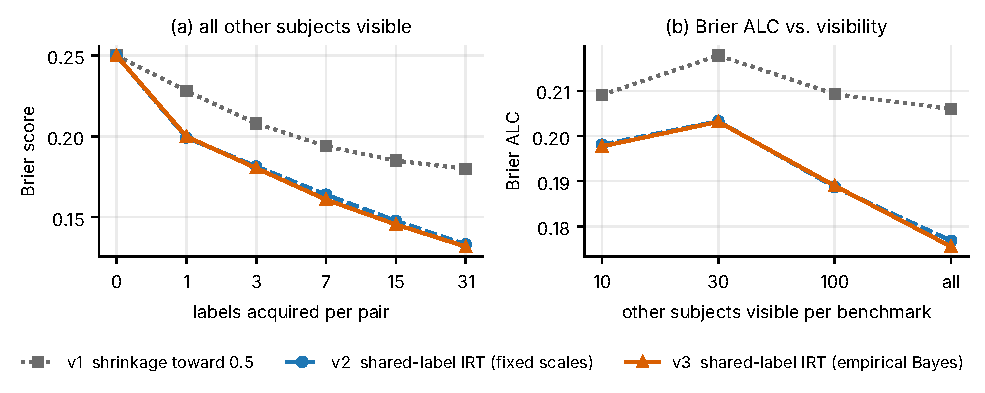
\includegraphics[width=0.97\linewidth]{figures/results.pdf}
\caption{Simulated results. (a) Brier score by label budget when all other subjects of the benchmark are visible. The zero-label point is $0.25$ for all methods. (b) Brier ALC against the number of visible subjects; the non-monotone shape comes from the changing benchmark set (see Section~\ref{sec:data}).}
\label{fig:res}
\end{figure}

\begin{table}[h]
\centering
\caption{Simulated Brier by budget, all subjects visible.}
\label{tab:budget}
\begin{tabular}{lcccccc}
\toprule
Method & $B_0$ & $B_1$ & $B_3$ & $B_7$ & $B_{15}$ & $B_{31}$ \\
\midrule
v1 & 0.2500 & 0.2281 & 0.2079 & 0.1939 & 0.1849 & 0.1799 \\
v2 & 0.2500 & 0.1992 & 0.1814 & 0.1639 & 0.1477 & 0.1332 \\
v3 & 0.2500 & 0.1999 & 0.1803 & 0.1608 & 0.1455 & 0.1317 \\
\bottomrule
\end{tabular}
\end{table}

\subsection{Ideas that did not help}
\label{sec:negative}
Table~\ref{tab:neg} lists the extensions we evaluated in the same simulator. Differences are changes in Brier ALC relative to the stated comparator (negative is better), at 30 visible subjects and with all visible.

\begin{table}[h]
\centering
\caption{Negative or negligible results. $\Delta$ is the change in simulated Brier ALC, negative being an improvement.}
\label{tab:neg}
\begin{tabular}{p{6.2cm}cc}
\toprule
Extension (comparator) & $\Delta$ ($S{=}30$) & $\Delta$ (all) \\
\midrule
Item-text prior from embeddings, best setting (IRT 1.0/1.5; embedded sample) & $-0.0013$ & $-0.0006$ \\
Subject-name ability prior (IRT 1.25/2.0) & $-0.0001$ & $+0.0009$ \\
Latent factors, rank 2, $\tau_f{=}0.75$ (IRT 1.25/2.0) & $-0.0000$ & $+0.0003$ \\
Latent factors, rank 2, $\tau_f{=}1.5$ (IRT 1.25/2.0) & $+0.0046$ & $+0.0153$ \\
Acquisition: items without any label first (random) & $-0.0004$ & $-0.0006$ \\
Acquisition: items with at most one label first (random) & $-0.0001$ & $-0.0007$ \\
Acquisition: already-seen items first (random) & $+0.0007$ & $+0.0153$ \\
Constant for zero labels, $0.55$ instead of $0.5$ & \multicolumn{2}{c}{$-0.00015$} \\
\bottomrule
\end{tabular}
\end{table}

\paragraph{Item text.} We embedded 282{,}564 item texts with \texttt{multilingual-e5-small} \citep{wang2024multilingual} (384 dimensions, texts built from the item features and content). A ridge regression trained on other benchmarks to predict item difficulty did not give a usable signal, and cosine similarity is high even across benchmarks (mean 0.81, against 0.89 within a benchmark), which suggests that the embeddings mostly encode the benchmark rather than the difficulty of an item. Within a benchmark, adding the embedding as a prior on $d_j$ gave at best $-0.0013$ with 30 visible subjects and $-0.0006$ with all visible, measured on the subsample of items that have embeddings. We did not submit it: the gain is small relative to our uncertainty, and it would require running a text encoder at test time.

\paragraph{Names and latent factors.} A prior on the ability from the model name (an ability table learnt on other benchmarks) and rank-2 latent factors both failed to help and the latter overfit when the factor prior was loose.

\paragraph{Acquisition.} Asking first for items that no other subject has labelled yet improves the simulation by under 0.001, because it widens the coverage of evaluation items by shared difficulty estimates (84\% against 78\% with all visible). The gain is within what we consider noise for a single run, and a custom \texttt{labeling.py} introduces a failure mode, so we kept the default policy. Asking for already-seen items first is much worse.

\section{Limitations}
\label{sec:limits}
(i) The simulator is our own reading of the rules. It treats the target as the mean response of an item and it assumes a given number of visible subjects. The number of subjects visible in the hidden test is unknown to us, and the feedback scores are too noisy to calibrate the simulator against them (Table~\ref{tab:real}). (ii) At budget 0 our simulation assumes no information and scores $0.25$. The submitted model would use labels of the same benchmark if the evaluator provides them at budget 0, which we could not check. (iii) The model relies on \texttt{labeled} containing labels of other subjects; if an evaluator restricted it to the target pair, the model reduces to the v1 behaviour. (iv) Non-binary benchmarks were dropped from our experiments, and the model ignores any revealed label that is not 0 or 1, so a benchmark with graded responses would receive the prediction 0.5. (v) Hyperparameters were selected on the same simulation as the comparisons, and there are no confidence intervals. The second stage is trained on episodes from our own simulator: cross-validation over benchmarks protects against overfitting to particular benchmarks, but not against a mismatch between the simulator and the real evaluation protocol (for example in the number of visible subjects or in how many labels the other subjects have), and the choice among three variants of it was made on the same folds. (vi) We only use binary outcomes; items with several trials are collapsed to their mean in the simulation.

\section{Reproducibility and disclosures}
\label{sec:repro}
\paragraph{Code and data.} The released repository contains the four submitted models, the build script of the submission ZIP, the experiment scripts (written for Kaggle notebooks, from data preparation to the second stage) and the result tables used in this report: \url{https://github.com/super-denis/paiec-2026-shared-label-irt}. The final submission ZIP contains \texttt{model.py} and \texttt{stack\_model.json} (the trees, 170~kB) and has no \texttt{requirements.txt} or \texttt{models.txt}; the trees are produced by \texttt{cell14.py}. The final Codabench submission ID is 1019684.

\paragraph{Training sources.} Only the public \texttt{measurement-db}; the trees of v4 are fitted on episodes simulated from it. No data outside it, and no data from the hidden test, were used.

\paragraph{Pretrained models.} The submitted predictor uses no pretrained model. \texttt{multilingual-e5-small} was used only in the experiments of Section~\ref{sec:negative}.

\paragraph{LLM assistance.} The code, the simulation and a first draft of this report were produced with the help of an LLM coding assistant (Claude, Anthropic) used through Claude Code, under the author's direction. The author ran all Kaggle experiments, submitted to Codabench and is responsible for the content.

\bibliographystyle{plainnat}
\begin{thebibliography}{9}
\bibitem[Brier(1950)]{brier1950}
G.~W. Brier.
\newblock Verification of forecasts expressed in terms of probability.
\newblock \emph{Monthly Weather Review}, 78(1):1--3, 1950.

\bibitem[Efron and Morris(1973)]{efron1973stein}
B.~Efron and C.~Morris.
\newblock Stein's estimation rule and its competitors: an empirical Bayes approach.
\newblock \emph{Journal of the American Statistical Association}, 68(341):117--130, 1973.

\bibitem[Polo et~al.(2024)]{polo2024tiny}
F.~M. Polo, L.~Weber, L.~Choshen, Y.~Sun, G.~Xu, and M.~Yurochkin.
\newblock tinyBenchmarks: evaluating {LLMs} with fewer examples.
\newblock In \emph{International Conference on Machine Learning}, 2024.

\bibitem[Rasch(1960)]{rasch1960}
G.~Rasch.
\newblock \emph{Probabilistic Models for Some Intelligence and Attainment Tests}.
\newblock Danish Institute for Educational Research, 1960.

\bibitem[Wang et~al.(2024)]{wang2024multilingual}
L.~Wang, N.~Yang, X.~Huang, L.~Yang, R.~Majumder, and F.~Wei.
\newblock Multilingual E5 text embeddings: a technical report.
\newblock \emph{arXiv:2402.05672}, 2024.
\end{thebibliography}

\appendix
\section{Implementation details}
\label{app:impl}
The model for one benchmark is fitted by repeating, for 24 sweeps (20 in v2), the Newton updates
\begin{align*}
c &\leftarrow c + \frac{\sum_i (y_i - p_i) - c/\tau_c^2}{\sum_i p_i(1-p_i) + 1/\tau_c^2},\\
a_s &\leftarrow a_s + \frac{\sum_{i\in s}(y_i - p_i) - a_s/\tau_a^2}{\sum_{i\in s}p_i(1-p_i) + 1/\tau_a^2},\qquad
d_j \leftarrow d_j + \frac{\sum_{i\in j}(y_i - p_i) - d_j/\tau_d^2}{\sum_{i\in j}p_i(1-p_i) + 1/\tau_d^2},
\end{align*}
recomputing $p_i=\sigma(c+a_{s_i}+d_{j_i})$ before each block. The clipping interval for the empirical Bayes scales is $[0.6,3]$ and $\tau_c=1.5$. A query returns $\sigma(c + a_s + d_j)$ clipped to $[0.02,0.98]$, with $a_s=0$ for an unseen subject and $d_j=0$ for an unseen item. The fit for a (benchmark, number of revealed labels) pair is cached.

\section{Features of the second stage}
\label{app:feat}
Let $\hat p_i=\sigma(c+a_{s_i}+d_{j_i})$ at the fitted values, $r_i=y_i-\hat p_i$ and $w_i=\hat p_i(1-\hat p_i)$ over the revealed labels. For the item $j$ of the query and the subject $s$: $\text{step\_item}_j=\sum_{i\in j} r_i a_{s_i}\,/\,(1+\sum_{i\in j} w_i a_{s_i}^2)$, $\text{step\_subj}_s=\sum_{i\in s} r_i d_{j_i}\,/\,(1+\sum_{i\in s} w_i d_{j_i}^2)$, $\text{corr\_item}=a_s\,\text{step\_item}_j$, $\text{corr\_subj}=d_j\,\text{step\_subj}_s$ and $\text{res\_item}_j=\sum_{i\in j} r_i/(1+n_j)$, all set to zero for an item without label. The other features are listed in Section~\ref{sec:methods}; the exact definitions are in \texttt{experiments/cell14.py} and are recomputed identically by \texttt{model.py} (checked to agree to machine precision).

\section{Reproducing the experiments}
\label{app:rep}
The experiment scripts are numbered \texttt{cell01.py} to \texttt{cell11.py}. Cell 1 downloads and compacts the binary benchmarks, cells 3 and 4 build item texts and embeddings, cell 5 tests item-level text models, cell 6 fits and exports the parameters of v1, cell 7 simulates shared labels, cells 8 to 11 give the experiments of this report (text prior, name prior and latent factors, acquisition policies, empirical Bayes scales), and cells 13 and 14 train and cross-validate the second stage (Table~\ref{tab:stack} comes from cell 14). Table~\ref{tab:sim} comes from cell 11, Table~\ref{tab:neg} from cells 8 to 10, and the files in \texttt{results/} are the raw outputs. The scripts expect the compacted data produced by cell 1 as a Kaggle input and run on CPU, except cell 4 (GPU), and all use a fixed seed.

\end{document}
